\documentclass{article}
\usepackage[utf8]{inputenc}
\usepackage[spanish]{babel}
\usepackage{graphicx}
\usepackage{listings}


\title{Informe Parcial II}
\author{daniel.perez19 }
\date{September 2021}

\begin{document}

\begin{titlepage}
    \begin{center}
        \vspace*{1cm}
            
        \Huge
        \textbf{Informe Parcial 2}
            
        \vspace{0.5cm}
        \LARGE
        Informática II
            
        \vspace{1.5cm}
            
        \textbf{Daniel Perez Gallego CC. 1193088770\\Jorge Montaña Cisneros CC.  1007327968}
            
        \vfill
            
        \vspace{0.8cm}
            
        \Large
        Departamento de Ingeniería Electrónica y Telecomunicaciones\\
        Universidad de Antioquia\\
        Medellín\\
        Septiembre de 2021
            
    \end{center}
\end{titlepage}

\tableofcontents
\vspace{2cm}
\section{Clases implementadas}
\subsection{Imagen}
Encargada de manejar la imagen con los parámetros de su alto y ancho\\
\subsection{Pixel RGB}
Es la encargada de almacenar los pixeles RGB de la imagen para luego separarlos\\

\section{Esquema de las clases}

\section{Código}

\section{Estructura del circuito montado}
Para la matriz de LEDs en Tinkerdad, diseñamos un circuito de 16x16 LEDs, hecha con tiras de neopixel. Cada una con su salida conectada a la entrada de la fila/tira superior, la potencia conectada a un sumnistro de energía y todas las coneciones para que el circuito funcione con normalidad\\

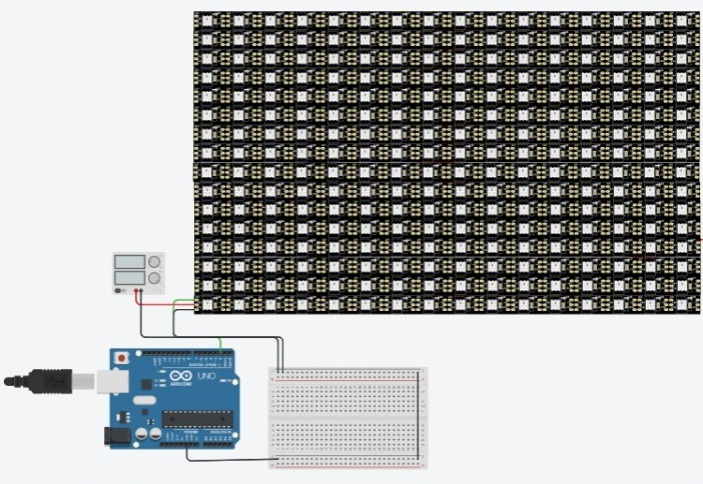
\includegraphics[width=14cm]{Imagenes/circuito.jpeg}

\section{Problemas presentados}
Justo como lo analizamos, el método para reducir y amplificar la imgagen fué la parte más complicada en la implementación, a pesar de que buscamos varias métodos, a la hora de codificarlo se complicaba y comenzamos a buscar un método para simplificarlo, hasta el punto donde consideramos aplicar un nuevo método y empezar casi desde 0.\\

Desconocíamos el formato que debían ser escritos los RGB en el .txt generado para tinkercad y si teníamos que insertar algún método para que el usuario no tenga que copiar y pegar el RGB en el tinkercad\\

La conexión del circuito fué un problema menor gracias a la búsqueda de documentación y videos sobre el código y la conexión en tinkercad; sin embargo, pensábamos que se encenderían los LEDs rápido, pero como no lo hacian debido a toda la información que se procesaba, abortabamos el proceso pensando que el circuito estaba malo, pero no lo estaba, solo éramos muy impacientes. 


\end{document}